\section{Method}
\subsection{Overview}

\begin{figure}[tb]
	\centering
	\begin{subfigure}{0.49\linewidth}
		\centering
		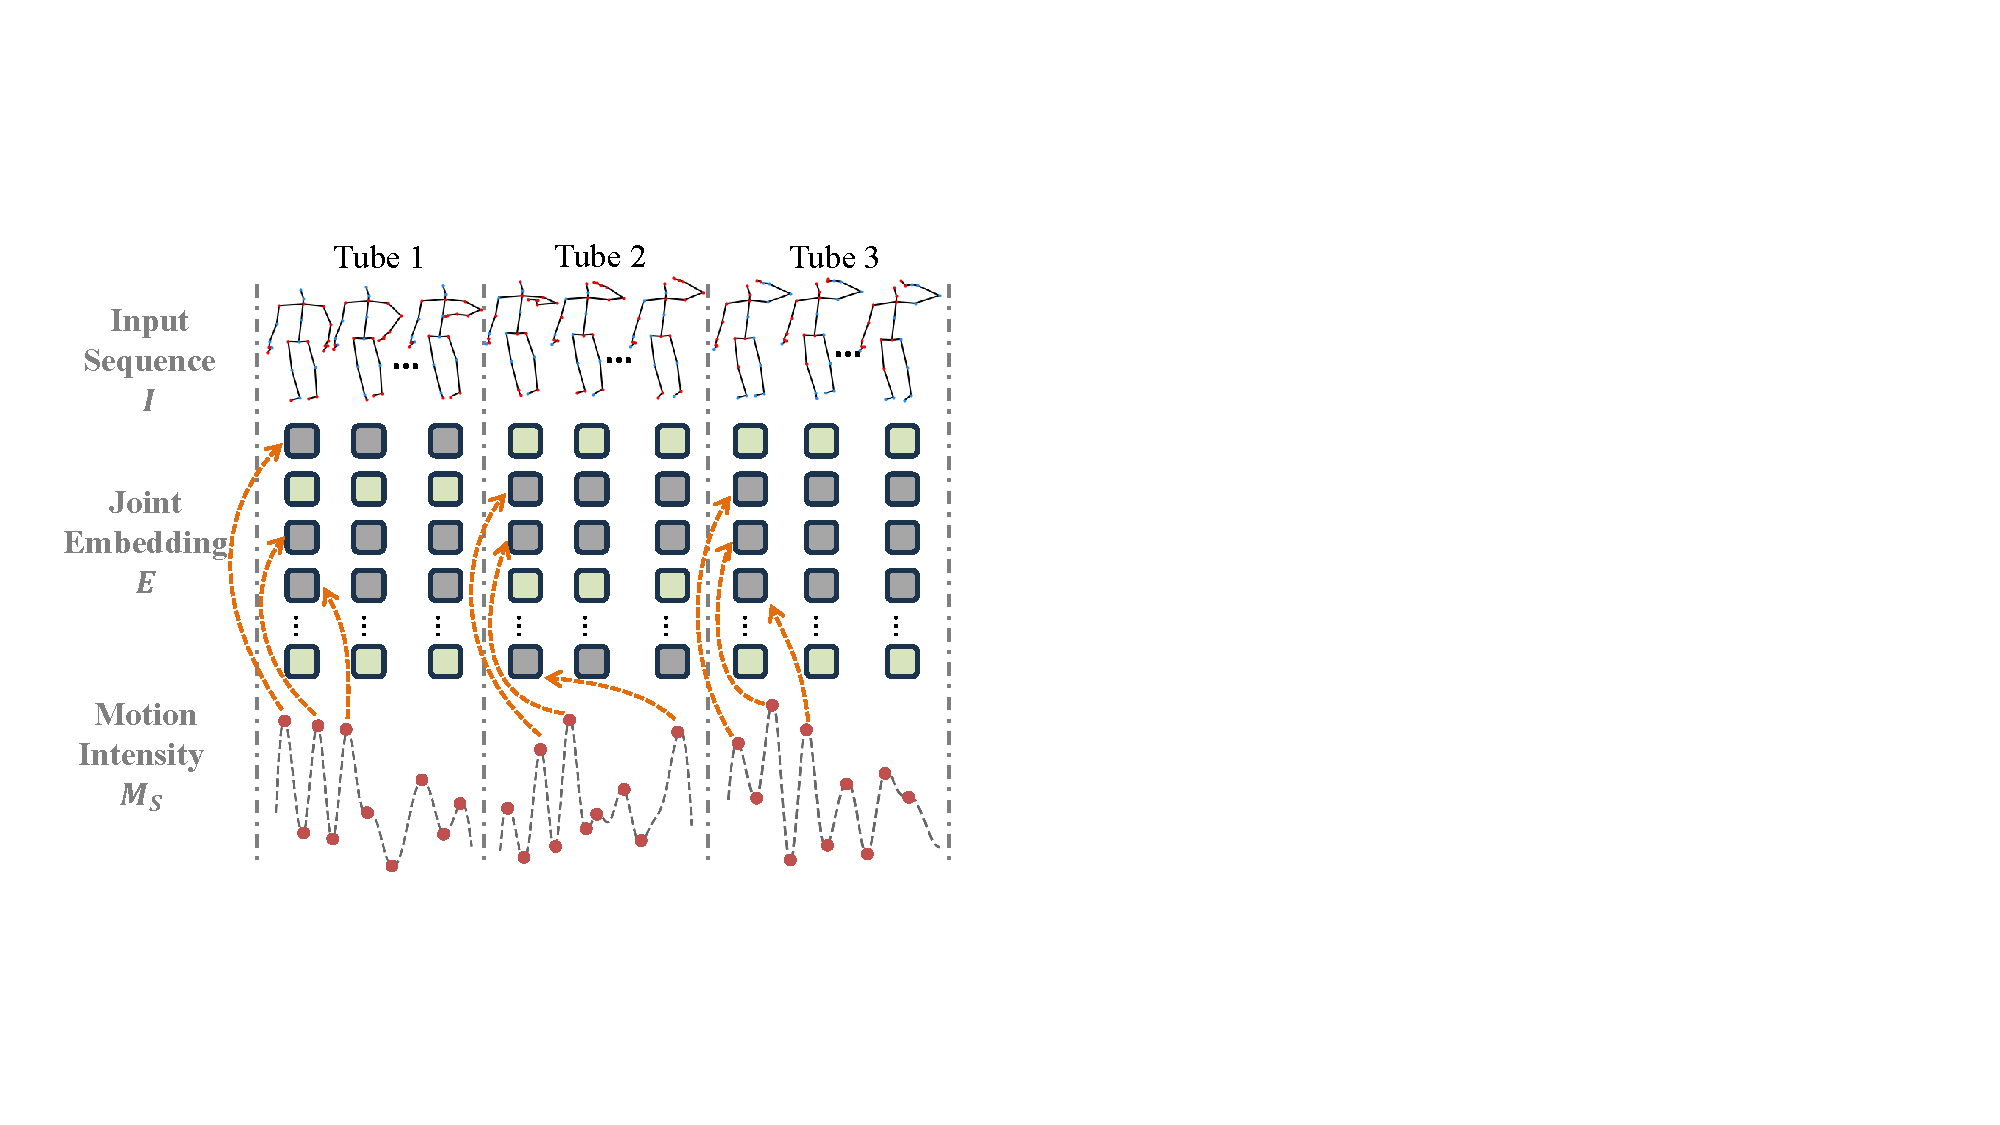
\includegraphics[width=0.95\linewidth]{figures/fig2_motion_aware_tube_masking.pdf}
		\caption{Motion-Aware Multi-Tube Masking}
		\label{fig2:motion_aware_tube_masking}
	\end{subfigure}
	\centering
	\begin{subfigure}{0.49\linewidth}
		\centering
		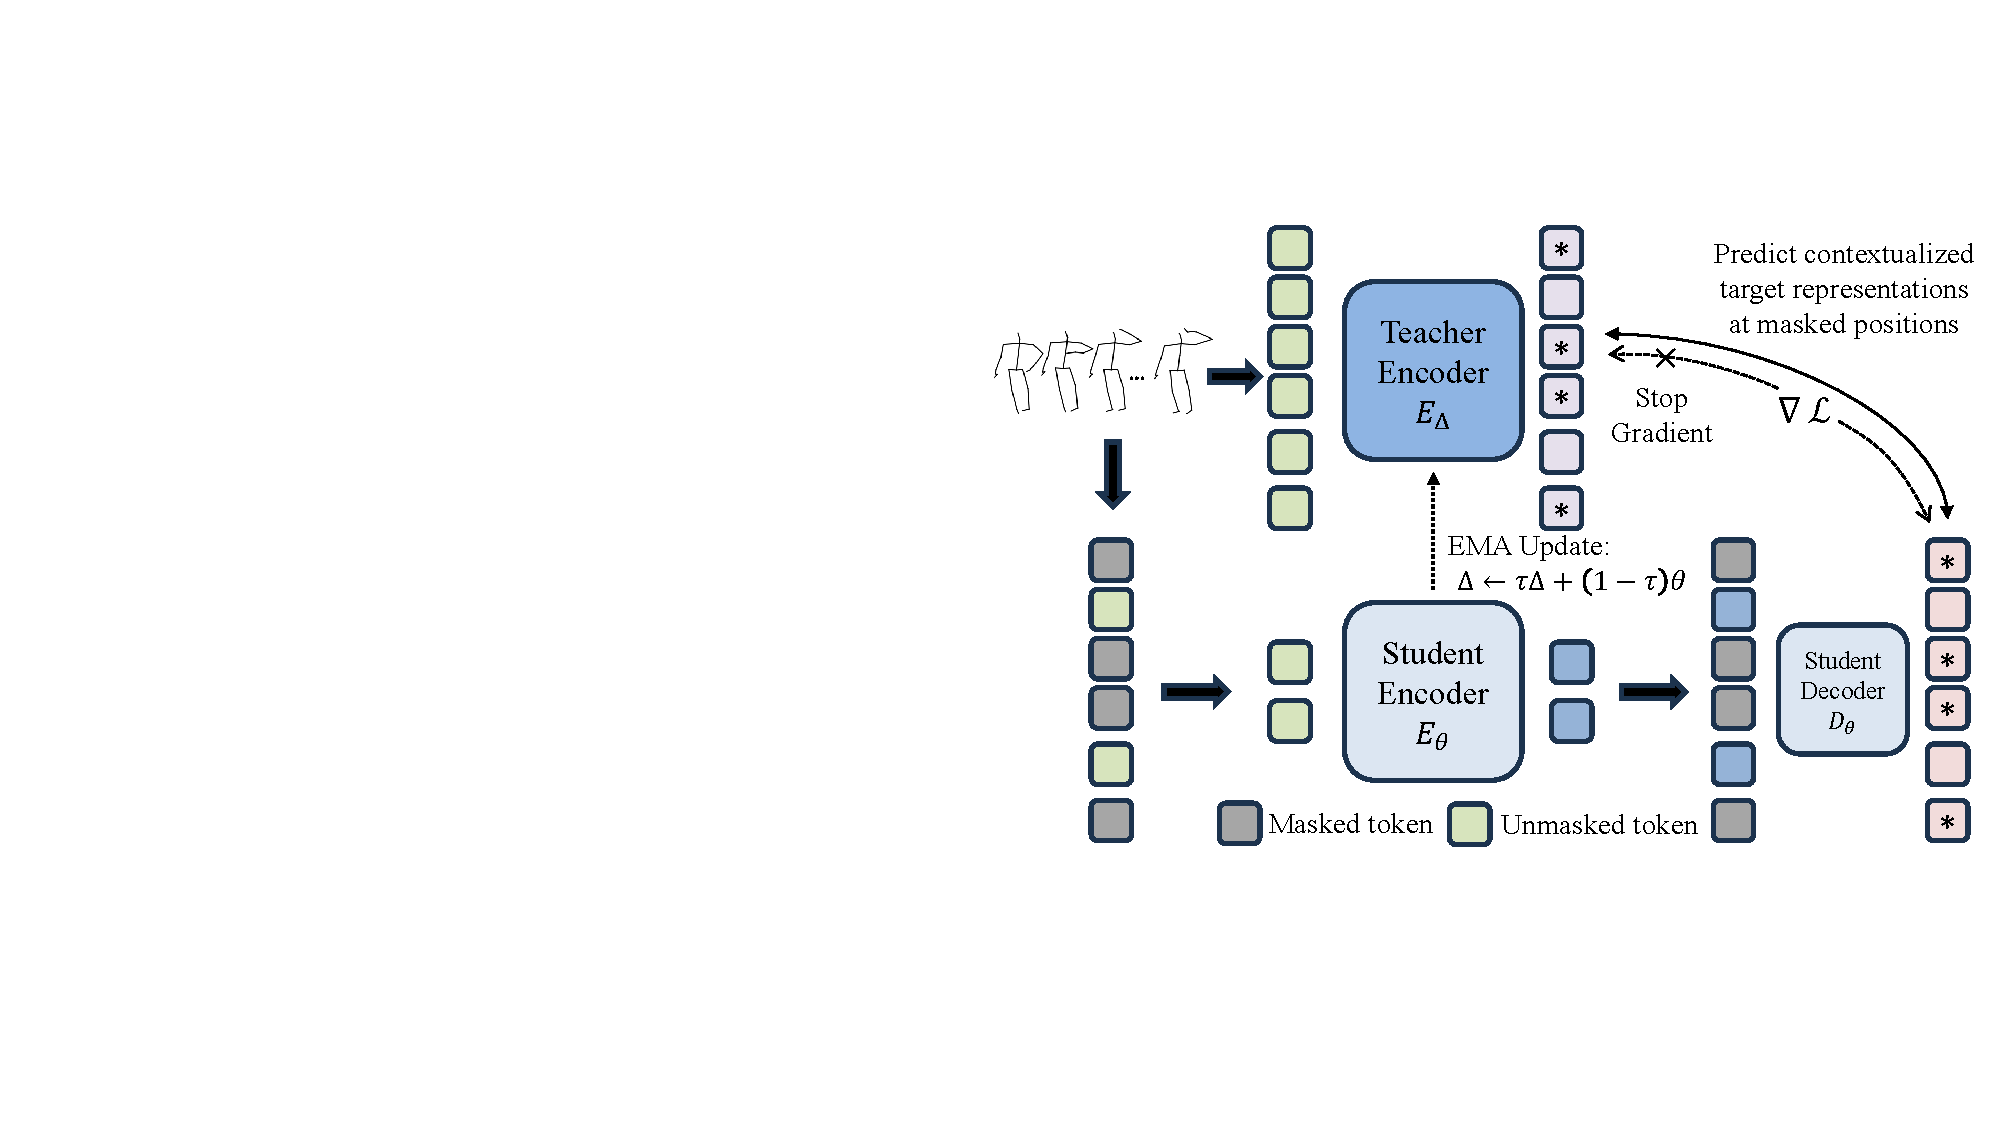
\includegraphics[width=0.95\linewidth]{figures/fig2_skeleton2vec.pdf}
		\caption{Skeleton2vec}
		\label{fig2:skeleton2vec}
	\end{subfigure}
    \caption{
    The overall pipeline of the proposed Skeleton2vec framework.
    We adopt the motion-aware multi-tube masking strategy (a) to guide the masking process,
    which prevents information leakage between adjacent frames and allows the model
    to focus more on semantically rich regions of motion. Subsequently, the teacher
    encoder $E_{\Delta}$ receives unmasked samples to construct latent contextualized targets,
    while the student encoder $E_{\theta}$ receives masked versions of the samples
    and predicts corresponding representations at the masked positions.
    }
    \label{fig2}
\end{figure}

The overall framework of Skeleton2vec is shown in \cref{fig2}.
It takes a skeleton sequence $I \in \mathbb{R}^{T_{s} \times V \times C_{s}}$ as
input, where $T_{s}$ is the the number of frames,
$V$ is the number of joints, and $C_{s}$ is the
the coordinates of joints.
Similar to most visual transformers \cite{dosovitskiy2020image},
the skeleton sequence is first divided into fixed-size patches and then linearly
transformed into patch embedding $E \in \mathbb{R}^{T_{e} \times V \times C_{e}}$.
After that, we employ the motion-aware multi-tube masking strategy to guide the masking of
joints. The teacher model constructs the full contextualized prediction targets
using unmasked training samples, while the student model receives the masked version
of the samples and predicts corresponding representations at the masked positions.

As our student model, we adopt an asymmetric encoder-decoder architecture, where the
encoder operates solely on non-masked tokens. The lightweight decoder inserts masked
tokens into the latent representations outputted by the encoder, forming a full set
for predicting the targets.
The teacher encoder shares the same model structure as the student. After accomplishing
the aforementioned pre-training task, the teacher encoder is retained for downstream task fine-tuning.

\subsection{Model Architecture}
\noindent \textbf{Encoder:}
Following MAMP \cite{mao2023masked}, we first divide the raw skeleton sequence
$I \in \mathbb{R}^{T_{s} \times V \times C_{s}}$ into non-overlapping segments
$I' \in \mathbb{R}^{T_{e} \times V \times (l \cdot C_{s})}$, where $T_{e}=T_{s}/l$
and $l$ is the length of each segment.
A trainable linear projection is then applied to each joint to obtain the embedding:
\begin{equation}
    \label{eq:joint_embedding_1}
    E_{j} = \text{LinearProj}(I') \in \mathbb{R}^{T_{e} \times V \times C_{e}},
\end{equation}
where $C_{e}$ represents the dimension of the embedding.
Temporal positional embedding $E_{t} \in \mathbb{R}^{T_{e} \times 1 \times C_{e}}$
and spatial positional embedding $E_{s} \in \mathbb{R}^{1 \times V \times C_{e}}$
are then added to the joint embedding to yield the final input:
\begin{equation}
    \label{eq:joint_embedding_2}
    E = E_{j} + E_{t} + E_{s},
\end{equation}

For the teacher encoder, the entire set is flattened as input $E^{T} \in \mathbb{R}^{N_{T} \times C_{e}}$,
where $N_{T}=T_{e} \times V$ represents the total number of tokens in the
skeleton sequence. For the student encoder, most tokens are masked, and
only the unmasked tokens are utilized as input, flattened as $E^{S} \in \mathbb{R}^{N_{S} \times C_{e}}$,
where $N_{S}=T_{e} \times V \times (1-m)$ denotes the number of visible tokens,
and $m$ is the masking ratio. 
Subsequently, $L_{e}$ layers of vanilla transformer blocks are applied to extract
latent representations. Each block comprises a multi-head self-attention (MSA)
module and a feed-forward network (FFN) module. Residual connections are employed
within each module, followed by layer normalization (LN).

\noindent \textbf{Decoder:} The decoder input
$D \in \mathbb{R}^{T_{e} \times V \times C_{e}}$ contains the full set of tokens,
including the latent representations of visible encoded tokens $Z^{S}_{e}$ and the inserted masked tokens.
Each masked token is represented by a shared learnable vector $E_{M} \in \mathbb{R}^{C_{e}}$,
indicating missing information to be predicted at that position. Similar to the
encoder, spatial positional embedding $E'_{s}$ and temporal positional embedding
$E'_{t}$ are added to all tokens to assist masked tokens in locating their positions.
The decoder employs an additional $L_{d}$ layers of transformer blocks for masked prediction.

\subsection{Contextualized Target Prediction}
Rather than relying on isolated raw joints or temporal motion with limited local context, we employ a
transformer-based teacher encoder to construct globally contextualized prediction targets,
thereby introducing a diverse training task.

\noindent \textbf{Contextualized Target Representations:}
We extract features from the output of each FFN block in every layer of the
teacher encoder and average them to form our training targets. Following data2vec 2.0
\cite{baevski2023efficient}, the features from each layer are normalized with
instance normalization \cite{ulyanov2016instance} before averaging.
Finally, the averaged features are normalized by layer normalization to serve as
the prediction targets. Normalizing the targets helps prevent the model from
collapsing to a trivial solution, and also prevents any single layer's features
from dominating. The generation of the target representations can be formulated as:
\begin{equation}
    \label{eq:target_rep}
    \begin{aligned}
        Y' &= \frac{1}{L_e}\sum_{l=1}^{L_e} \text{IN}(Z_l^T), \\
        Y &= \text{LN}(Y'),
    \end{aligned}
\end{equation}
where IN and LN refer to instance normalization and layer normalization, respectively.
$Z_l^T$ denotes the output of the FFN block in the $l^{th}$ layer of the teacher encoder.

\noindent \textbf{Target Prediction:}
Given the output $H_d$ of the student decoder, we employ an additional linear prediction head to
regress the contextualized target representations of the teacher:  
\begin{equation}
    \label{eq:target_pred}
    \hat{Y} = \text{LinearPred}(H_d),
\end{equation}

Finally, we adopt L2 loss as our learning objective, calculating loss only for the
masked positions:
\begin{equation}
    \label{eq:loss}
    \mathcal{L} = \frac{1}{|\mathcal{M}|}\sum_{i \in \mathcal{M}}||Y_i - \hat{Y}_i||_2^2,
\end{equation}
where $\mathcal{M}$ denotes the set of masked positions.

\noindent \textbf{Teacher Parameterization:}
The student model weights $\theta$ are updated through backpropagation on the loss
gradients. The teacher model weights $\Delta$ are initialized to be the same as the
student weights and parameterized during training by taking an exponentially moving
average (EMA) of the student weights:  
\begin{equation}
    \label{eq:ema}
    \Delta \leftarrow \tau\Delta + (1-\tau)\theta,
\end{equation}
where $\tau$ is a hyperparameter controlling the update frequency of the teacher
weights using a linearly increasing schedule, gradually increasing from an initial
value $\tau_0$ to 1 throughout training.

\subsection{Motion-Aware Multi-Tube Masking}
\label{sec:motion-aware_tube_masking}
We propose the motion-aware multi-tube masking strategy to address the issue of high
spatiotemporal correlations in skeleton sequences.

\noindent \textbf{Multi-Tube Division:}
The tube masking strategy, initially introduced by VideoMAE \cite{tong2022videomae},
considers the entire video sequence along the temporal axis as a single tube,
sharing the same masking map across different frames. This mitigates the information
leakage issue between adjacent frames.
Although the skeleton sequence is derived from the
video, directly applying this single-tube
masking strategy to skeleton data is suboptimal due to the inherent structural differences.
In video data, the basic units for masking are image patches in each frame. Due to scene
motion or camera viewpoint changes, a masked body part like the hand in the first frame
may find its correspondence in unmasked regions in later frames far apart, which facilitates
long-range dependency modeling.
In contrast, the basic units for masking in skeleton sequences
are the joints in each skeleton frame, where the same-order joints have explicit correspondence
across frames. As a result, a body part masked in the first skeleton frame will remain
masked in all frames, causing a complete loss of information for that part, which makes
the masked prediction task overly difficult and harms the model's learning capability.
To address this, as illustrated in \cref{fig2:motion_aware_tube_masking},
we empirically divide the skeleton sequence along the time axis into multiple tubes
instead of one tube. Each tube shares the same masking map to force the model to extract
information from farther time steps, while different tubes use different masking maps
to avoid joints being masked throughout.
The comparison between random masking, single-tube masking, and our
multi-tube masking is visually depicted in \cref{fig:masking_cmp}.
The tube division can be represented as:
\begin{equation}
    \label{eq:deviding_tubes}
    E'=\text{Reshape}(E) \in \mathbb{R}^{N \times \alpha \times V \times C_{e}}, 
\end{equation}

\noindent where $\alpha$ is tube length and $N=\frac{T_{e}}{\alpha}$ is number of tubes.

\noindent \textbf{Motion-Aware Sampling:}
Regions with larger motion intensity intuitively contain richer semantic information
about actions. Therefore, we utilize the spatial motion intensity of each human body
joint within a tube as empirical guidance to generate the masking map.

Specifically, we first extract the corresponding motion sequence
$M \in \mathbb{R}^{T_{s} \times V \times C_{s}}$ from the input skeleton sequence
$I \in \mathbb{R}^{T_{s} \times V \times C_{s}}$ by calculating temporal differences
of corresponding joint coordinates between adjacent frames:
\begin{equation}
    \label{eq:motion}
    M_{i,:,:} = \begin{cases} 
    I_{i+1,:,:}-I_{i,:,:}, & i \in 0, \dots, T_{s}-1\\
    0, & i=T_{s}  
\end{cases}
\end{equation}

Similar to joint embedding in the encoder, we reshape $M$ into non-overlapping
segments $M' \in \mathbb{R}^{T_{e} \times V \times (l \cdot C_{s})}$ to match the
shape of input sequence $I'$. We then calculate the motion intensity of each joint
within a segment as:
\begin{equation}  
    \label{eq:motion_intensity}
    S_{i,:} = \sum_{k=0}^{l\cdot C_{s}}|M'_{i,:,k}| \in \mathbb{R}^{T_{e} \times V}, \quad i=0,\dots,T_{e}
\end{equation}

Afterwards, we compute the spatial motion intensity of each body joint within a tube,
normalizing it along the spatial dimension:  
\begin{equation}
    \label{eq:tube_motion_intensity_norm}
    \begin{aligned}
        T_{i,:} &= \sum_{j=i}^{i+\alpha}S_{j,:} \in \mathbb{R}^{N \times V}, \quad &i=0,\dots,N \\
        T'_{i,:} &= T_{i,:} / \text{max}(T_{i,:}), \quad &i=0,\dots,N  
    \end{aligned}
\end{equation}

Finally, we utilize the normalized spatial motion intensity to generate a unique
masking map for each tube:
\begin{equation} 
    \label{eq:mask_sampling}
    \begin{aligned}
        p &= \eta + \beta \cdot T', \quad &\eta \sim U(0,1) \\  
        \mathcal{M}_{i} &= \text{argsort}(p_{i,:})[-K:], \quad &i=0,\dots,N
    \end{aligned}
\end{equation}

\noindent where $\eta$ is random noise drawn from a uniform distribution between
0 and 1, $\beta$ is a hyperparameter controlling the influence of spatial motion
intensity on sampling, $\mathcal{M}_{i}$ is the masking map for $i^{th}$ tube,
$K=V\times (1-m)$ is the number of joints to be masked, and $m$ is the masking ratio.
By customizing motion-aware masking maps for each tube, the model is encouraged
to focus more on semantically richer regions, leading to improved spatiotemporal representations.


